%%% Figure from: Schär, Fabian. "Blockchain Forks: A Formal Classification Framework and Persistency Analysis." (2020). 

\begin{table}[h!]
\center
  \begin{tabular}{ccc}
  \hline \hline
     & \scriptsize $S_{new}$ dominant ($r_{new}>r_{old}$) & \scriptsize $S_{old}$ dominant ($r_{new}<r_{old}$)\\ \cline{2-3}
     &&\\
    Soft fork & %($S_{new} \subset S_{old}$)&
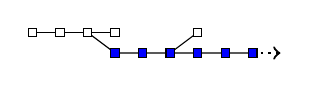
\begin{tikzpicture}[domain=1:10,scale=0.35, every node/.style={scale=0.35}]
\coordinate (o1) at (1,1);
\coordinate (o2) at (2,1);
\coordinate (o3) at (3,1);
\coordinate (o4) at (4,1);
\coordinate (o5) at (5,1);
\coordinate (o6) at (6,1);
\coordinate (o7) at (7,1);
\coordinate (o8) at (8,1);
\coordinate (o9) at (9,1);
\coordinate (o10) at (10,1);
\coordinate (n1) at (1,0.25);
\coordinate (n2) at (2,0.25);
\coordinate (n3) at (3,0.25);
\coordinate (n4) at (4,0.25);
\coordinate (n5) at (5,0.25);
\coordinate (n6) at (6,0.25);
\coordinate (n7) at (7,0.25);
\coordinate (n8) at (8,0.25);
\coordinate (n9) at (9,0.25);
\coordinate (n10) at (10,0.25);

  \draw[] (o1) to[] (o2) to[] (o3) to[] (o4);
  \draw[] (o3) to[] (n4) to[] (n5) to[] (n6) to[] (n7) to[] (n8) to[] (n9);
  \draw[color=black] (n6) to[] (o7);
  %\draw[color=black,densely dashed] (o4) to[] (o5);
  %\draw[color=black,densely dashed] (o7) to[] (o8);
  \draw[color=black,thick, dotted, ->] (n9) to[] (n10);

  %\filldraw[draw=black,fill=white] (o1) circle (5pt);
  %\filldraw[draw=black,fill=white] (o2) circle (5pt);
  %\filldraw[draw=black,fill=white] (o3) circle (5pt);
  %\filldraw[draw=black,fill=white] (o4) circle (5pt);
  %\filldraw[draw=black,fill=white] (o5) circle (5pt);
  %\filldraw[draw=black,fill=white] (o6) circle (5pt);
  %\filldraw[draw=black,fill=white] (o7) circle (5pt);
  %\filldraw[draw=black,fill=white] (o8) circle (5pt);
  %\filldraw[draw=black,fill=white] (o9) circle (5pt);
  \node (rect) at (o1) [fill=white,draw,minimum width=0.3cm,minimum height=0.3cm] {};
  \node (rect) at (o2) [fill=white,draw,minimum width=0.3cm,minimum height=0.3cm] {};
  \node (rect) at (o3) [fill=white,draw,minimum width=0.3cm,minimum height=0.3cm] {};
  \node (rect) at (o4) [fill=white,draw,minimum width=0.3cm,minimum height=0.3cm] {};
  %\node (rect) at (o5) [fill=white,draw,minimum width=0.3cm,minimum height=0.3cm] {};
  %\node (rect) at (o6) [fill=white,draw,minimum width=0.3cm,minimum height=0.3cm] {};
  \node (rect) at (o7) [fill=white,draw,minimum width=0.3cm,minimum height=0.3cm] {};
  %\node (rect) at (o8) [fill=white,draw,minimum width=0.3cm,minimum height=0.3cm] {};
  %\node (rect) at (o9) [fill=white,draw,minimum width=0.3cm,minimum height=0.3cm] {};
  %\filldraw[draw=black,fill=blue] (n4) circle (5pt);
  %\filldraw[draw=black,fill=blue] (n5) circle (5pt);
  %\filldraw[draw=black,fill=blue] (n6) circle (5pt);
  %\filldraw[draw=black,fill=blue] (n7) circle (5pt);
  %\filldraw[draw=black,fill=blue] (n8) circle (5pt);
  %\filldraw[draw=black,fill=blue] (n9) circle (5pt);
  %\node (rect) at (n1) [fill=white,draw,minimum width=0.3cm,minimum height=0.3cm] {};
  %\node (rect) at (n2) [fill=white,draw,minimum width=0.3cm,minimum height=0.3cm] {};
  %\node (rect) at (n3) [fill=white,draw,minimum width=0.3cm,minimum height=0.3cm] {};
  \node (rect) at (n4) [fill=blue,draw,minimum width=0.3cm,minimum height=0.3cm] {};
  \node (rect) at (n5) [fill=blue,draw,minimum width=0.3cm,minimum height=0.3cm] {};
  \node (rect) at (n6) [fill=blue,draw,minimum width=0.3cm,minimum height=0.3cm] {};
  \node (rect) at (n7) [fill=blue,draw,minimum width=0.3cm,minimum height=0.3cm] {};
  \node (rect) at (n8) [fill=blue,draw,minimum width=0.3cm,minimum height=0.3cm] {};
  \node (rect) at (n9) [fill=blue,draw,minimum width=0.3cm,minimum height=0.3cm] {};
\end{tikzpicture}
    &
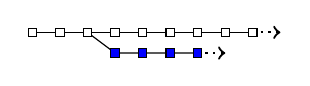
\begin{tikzpicture}[domain=1:10,scale=0.35, every node/.style={scale=0.35}]
\coordinate (o1) at (1,1);
\coordinate (o2) at (2,1);
\coordinate (o3) at (3,1);
\coordinate (o4) at (4,1);
\coordinate (o5) at (5,1);
\coordinate (o6) at (6,1);
\coordinate (o7) at (7,1);
\coordinate (o8) at (8,1);
\coordinate (o9) at (9,1);
\coordinate (o10) at (10,1);
\coordinate (n1) at (1,0.25);
\coordinate (n2) at (2,0.25);
\coordinate (n3) at (3,0.25);
\coordinate (n4) at (4,0.25);
\coordinate (n5) at (5,0.25);
\coordinate (n6) at (6,0.25);
\coordinate (n7) at (7,0.25);
\coordinate (n8) at (8,0.25);
\coordinate (n9) at (9,0.25);
\coordinate (n10) at (10,0.25);

  \draw[color=black] (o1) to[] (o2) to[] (o3) to[] (o4) to (o5) to (o6) to (o7) to (o8) to (o9);
  \draw[color=black] (o3) to[] (n4) to[] (n5) to[] (n6) to[] (n7);
  \draw[color=black,thick, dotted, ->] (o9) to[] (o10);
  \draw[color=black,thick, dotted, ->] (n7) to[] (n8);

  %\filldraw[draw=black,fill=white] (o1) circle (5pt);
  %\filldraw[draw=black,fill=white] (o2) circle (5pt);
  %\filldraw[draw=black,fill=white] (o3) circle (5pt);
  %\filldraw[draw=black,fill=white] (o4) circle (5pt);
  %\filldraw[draw=black,fill=white] (o5) circle (5pt);
  %\filldraw[draw=black,fill=white] (o6) circle (5pt);
  %\filldraw[draw=black,fill=white] (o7) circle (5pt);
  %\filldraw[draw=black,fill=white] (o8) circle (5pt);
  %\filldraw[draw=black,fill=white] (o9) circle (5pt);
  \node (rect) at (o1) [fill=white,draw,minimum width=0.3cm,minimum height=0.3cm] {};
  \node (rect) at (o2) [fill=white,draw,minimum width=0.3cm,minimum height=0.3cm] {};
  \node (rect) at (o3) [fill=white,draw,minimum width=0.3cm,minimum height=0.3cm] {};
  \node (rect) at (o4) [fill=white,draw,minimum width=0.3cm,minimum height=0.3cm] {};
  \node (rect) at (o5) [fill=white,draw,minimum width=0.3cm,minimum height=0.3cm] {};
  \node (rect) at (o6) [fill=white,draw,minimum width=0.3cm,minimum height=0.3cm] {};
  \node (rect) at (o7) [fill=white,draw,minimum width=0.3cm,minimum height=0.3cm] {};
  \node (rect) at (o8) [fill=white,draw,minimum width=0.3cm,minimum height=0.3cm] {};
  \node (rect) at (o9) [fill=white,draw,minimum width=0.3cm,minimum height=0.3cm] {};
  %\filldraw[draw=black,fill=blue] (n4) circle (5pt);
  %\filldraw[draw=black,fill=blue] (n5) circle (5pt);
  %\filldraw[draw=black,fill=blue] (n6) circle (5pt);
  %\filldraw[draw=black,fill=blue] (n7) circle (5pt);
  %\filldraw[draw=black,fill=blue] (n8) circle (5pt);
  %\filldraw[draw=black,fill=blue] (n9) circle (5pt);
  %\node (rect) at (n1) [fill=white,draw,minimum width=0.3cm,minimum height=0.3cm] {};
  %\node (rect) at (n2) [fill=white,draw,minimum width=0.3cm,minimum height=0.3cm] {};
  %\node (rect) at (n3) [fill=white,draw,minimum width=0.3cm,minimum height=0.3cm] {};
  \node (rect) at (n4) [fill=blue,draw,minimum width=0.3cm,minimum height=0.3cm] {};
  \node (rect) at (n5) [fill=blue,draw,minimum width=0.3cm,minimum height=0.3cm] {};
  \node (rect) at (n6) [fill=blue,draw,minimum width=0.3cm,minimum height=0.3cm] {};
  \node (rect) at (n7) [fill=blue,draw,minimum width=0.3cm,minimum height=0.3cm] {};
  %\node (rect) at (n8) [fill=white,draw,minimum width=0.3cm,minimum height=0.3cm] {};
  %\node (rect) at (n9) [fill=white,draw,minimum width=0.3cm,minimum height=0.3cm] {};
\end{tikzpicture}
\\
&&\\ \hline \hline
  \end{tabular}
\end{table}
